\documentclass[pdftex, 12pt, a4paper]{report}
\usepackage[backend=bibtex, style=authoryear, citestyle=authoryear, natbib=true]{biblatex}
\addbibresource{references.bib}
\usepackage[top=2.5cm, left=3cm, bottom=2.5cm, right=2cm]{geometry}
\newcommand{\defeq}{\mathrel{\mathop:}=}

\usepackage{graphicx}
\usepackage{float}
% For the code
\usepackage{listings}
\usepackage{color}
\usepackage{array}

% For the graphs
\usepackage{tikz}
\usetikzlibrary{arrows}

\definecolor{dkgreen}{rgb}{0,0.6,0}
\definecolor{gray}{rgb}{0.5,0.5,0.5}
\definecolor{mauve}{rgb}{0.58,0,0.82}

\lstset{frame=tb,
	aboveskip=3mm,
	belowskip=3mm,
	showstringspaces=false,
	columns=flexible,
	basicstyle={\small\ttfamily},
	numbers=none,
	numberstyle=\tiny\color{gray},
	keywordstyle=\color{blue},
	commentstyle=\color{dkgreen},
	stringstyle=\color{mauve},
	breaklines=true,
	breakatwhitespace=true,
	tabsize=6
}

\begin{document}
	
	\tableofcontents
	
	\chapter{Preface: Why this book?}	
	\section{Anatomy of a computable problem}
	
	Many computable problems can be solved with a process encapsulating \textit{four} components, with percentage indicating authors personal estimate on time spent on that particular step:
	
	\begin{enumerate}
		\item Problem formulation (60 \%)
		\item Finding the tools \ solving method (20 \%)
		\item Calculation (10\%)
		\item Interpretation (10 \%)
	\end{enumerate}
	
	Conrad Wolfram, the man behind this problem composition described current math education in this manner: 
	\begin{quote}
		"Now here's the crazy thing right now. In math education, we're spending about perhaps 80 percent of the time teaching people to do step three by hand. Yet, that's the one step computers can do better than any human after years of practice. Instead, we ought to be using computers to do step three and using the students to spend much more effort on learning how to do steps one, two and four -- conceptualizing problems, applying them, getting the teacher to run them through how to do that. (...)
	\end{quote}
	
	\begin{quote}
	 Basically, no one's very happy. Those learning it think it's disconnected, uninteresting and hard. Those trying to employ them think they don't know enough. Governments realize that it's a big deal for our economies, but don't know how to fix it. And teachers are also frustrated. Yet math is more important to the world than at any point in human history. So at one end we've got falling interest in education in math, and at the other end we've got a more mathematical world, a more quantitative world than we ever have had."
	\end{quote}
		
		
		Thanks to a environment encouraging self-motivation and a great teacher I found myself skipping the boundaries of traditional education system and set out to wonder the world by myself. When I encountered \textit{untamed} mathematics that was unrestricted by the classroom setting I was instantly hooked and have rarely if ever looked back. I hope that this composition of ideas will help many see mathematics just like I saw \textit{wild} math for the first time - with awe, admiration and love. \par
		
		Putting all the amazing, astonishing pieces of logic and beauty aside and we are still left with the fact that mathematics is just plain useful. Are you talking about searching cure for cancer, developing general purpose artificial intelligence or auto-tagging peoples faces on Facebook, math is there. It is not only beautiful put also very and I mean \textit{very}, useful. \par
		
		This book might not be the whole epic journey to pure math wizardry but might be a start for somebody. If it is for somebody out there - you made writing this worthwhile and I sincerely want to say: "Thank you for your time and effort!"
		
		The need for this book is here and we needed it yesterday. But as saying goes -- "Better late than never."
				
	
	
	\chapter{Power of estimation}
	
	\section{Beginning is somewhere here}
	Estimation is the main type of calculation I have encountered and is often not regarded as mathematics but the logic and techniques can be well quantified. Giving an estimate for the amount of time your computer will be running on a problem to the amount of paper cups you need for a party I feel this is the skill for everyone who is out there. \par
	
	Most important knowledge is the accuracy requirement on the problem. For example if you are calculating the motion of a ball off a ramp, you wouldn't really care if the ball rolled few centimeters further or not. But if the ball was from a game of pool and you estimated wrong then it could cost you the game because errors accumulate and winner is often only a bit better than the opponent. \par
	
	Also it can be helpful to know if you are looking an estimate for the under- or upper-bound. It can be very unpleasant if you do not have enough plates for all the guests when having a food orgy so when buying plates you give yourself a safety margin of few plates from the maximum number of guests you expect at a time. Overshooting your estimate -- just to be safe.
	
	\section{Fermi problems}
	\subsection{What are they?}
	Fermi problems are also often called back-of-the-envelope calculations and find to give quick and approximate answers. They are far from complete proofs or precise answers but provide close enough estimates to questions that then can be used accordingly. They are named after physicist Enrico Fermi who was known to give very quick and accurate estimations to complicated questions. For instance on the first atomic bomb test in New Mexico on 16th July 1945 he estimated the atomic bomb size by seeing how far pieces of paper fell from his hand due to blast wave. After calculations he reached estimate of 10 kilotons of TNT while the blast was measured 18 kilotons of TNT.
	\subsection{Examples}
	
	\subsubsection{Example 1. How many tennis balls would you need to fill a cement truck?}
	
	Lets take the example question: How many tennis balls would you need to fill a cement truck? I recall seeing a cement truck and it looked almost like a huge cylinder on the back, with about 2.5 meter diameter and with length of 4 meters. The whole volume of the truck could then be around $L \times r^2 \times \pi \approx 4 * 2.5^2 * 3 = 75 m^3$. Now to estimate the tennis balls volume I crunch my fist and say that tennis ball is about this big. My fist is around $12cm = 0.12m \approx 0.1m$ in diameter so the area of the ball is around $\frac{4}{3}\pi r^3 \approx \frac{4*3*0.001m^3}{3} = 4\times10^{-4}m^3$. Now for the amount of tennis balls all we need to do is divide: $75 / 0.004 \approx 19000$. (80 / 0.004 is 20000 and take a bit off, the real answer is 18750. I checked after, I promise!). That is my final answer - the real number is at the end of the section. So I will not spoil it for you. But the thing to notice is that the answer is relatively close. A lot better than it would be by blindly guessing.\newline
	
	\subsubsection{Example 2. How many handcuffs would it take in order to create an interlocked chain from the Earth to the Sun?}
	
	The pair of handcuffs is around 0.3 m in length. Harder part is estimating the distance between Earth and the Sun. I know that light from the Sun reaches Earth within 8 minutes and that light travels at the speed of around $3\times 10^8 m/s$. 8 minutes contains $8\times60 \approx 500$ seconds (I know that $9 \times 60$ would be 540). Therefore the distance is $500 \times 3 \times 10^8 m = 1.5 \times 10^{11}$. As $0.3 \approx \frac{1}{3}$ Number of handcuffs becomes distance divided by handcuff length: $1.5\times 10^{11} : \frac{1}{3} = 4.5 \times 10^{11}$. That is my final answer.\newline\newline
	
	\subsubsection{Practice Fermi problems}
	\begin{enumerate}
			\item What is 75 to the power of 9? 
			\item What number of M\&Ms would you have to lay on the surface area of a 24 inch beach ball in order to fully cover it? 
			\item How many toothpicks would fit in a basketball?
			\item How many grains of sand are there on all the beaches in the world combined?
			\item How many steps would it take an average human to travel from Stockholm to Mumbai?
			\item How many times larger is the largest acceleration to which a human volunteer has been subjected than the acceleration of a sneeze? 
	\end{enumerate}
	\newpage
	\subsubsection{Answers}
	
	Example 1. How many tennis balls would you need to fill a cement truck? 28700\newline
	You can calculate the real answer by looking at wikipedia pages for Circle, Circle packing, Close-packing of spheres, Concrete mixer and Tennis ball. \newline\newline
	
	\noindent Example 2. How many handcuffs would it take in order to create an interlocked chain from the Earth to the Sun?  $6.25 \times 10^{11}$\newline
	\noindent	http://www.wolframalpha.com/input/?i=earth+to+sun \newline
	https://www.ncjrs.gov/pdffiles1/nij/082981.pdf \newline\newline
	
	
	\noindent\textbf{Practice Fermi problems}
	\begin{enumerate}
		\item $7.508468628\times10^{16}$
		\item 7640
		\item 27300
		\item $10^{21}$
		\item $1.1\times10^7$
		\item 28.6
	\end{enumerate}

	\noindent All the questions are stolen from: http://www.fermiquestions.com/ \newline\newline
	Check it out, it is awesome!
	\subsection{Advanced: Estimating error of Fermi calculation}
	Fermi estimates generally work because the estimations of the individual terms are often close to correct, and overestimates and underestimates help cancel each other out. That is, if there is no consistent bias, a Fermi calculation that involves the multiplication of several estimated factors will probably be more accurate than might be first supposed. \par 
	
	In detail, multiplying estimates corresponds to adding their logarithms; thus one obtains a sort of Wiener process or random walk on the logarithmic scale, which diffuses as $\sqrt{n}$ (in number of terms n). In discrete terms, the number of overestimates minus underestimates will have a binomial distribution. In continuous terms, if one makes a Fermi estimate of n steps, with standard deviation $\sigma$ units on the log scale from the actual value, then the overall estimate will have standard deviation $\sigma^{\sqrt{n}}$, since the standard deviation of a sum scales as $\sqrt{n}$ in the number of summands. \par
	
	For instance, if one makes a 9-step Fermi estimate, at each step overestimating or underestimating the correct number by a factor of 2 (or with a standard deviation 2), then after 9 steps the standard error will have grown by a logarithmic factor of $\sqrt{9}=3$, so $2^3=8$. Thus one will expect to be within 1/8 to 8 times the correct value – within an order of magnitude, and much less than the worst case of erring by a factor of $2^9=512$ (about 2.71 orders of magnitude). If one has a shorter chain or estimates more accurately, the overall estimate will be correspondingly better. \par
	
	CITATION NEEDED, WIKIPEDIA, FERMI PROBLEM
	
	\section{Avoid time consuming algorithms}
	
	\section{This won't take long}
	
	We can often find very accurate solutions to problems without actually finding exact answers. 
	
	
	\subsection{Factorial - Stirling's approximation}
	
	One example would be using Stirling's formula instead of factorial. The larger the factorial we are trying to estimate the better the approximation. Stirling's formula is given by: $$n! \approx (\sqrt{2\pi n}) (\frac{n}{e})^n$$
	
	Where $\pi$ is circle constant approximately 3.141 and $e$ is another constant about 2.718.
	\begin{figure}[H]
	\begin{lstlisting}
		from math import factorial, sqrt, pi, e
		# Using stirling approximation approximate factorial function.
		# Very accurate after n > 1000
		# http://en.wikipedia.org/wiki/Stirling%27s_approximation
		
		def stirling(n):
			return sqrt(2*pi*n)*(n/e)**n
		
		s = stirling(100)
		f = factorial(100) * 1.0
		print("\n\nStirling approximation to 100! is:", s, "Compared to exact value of:", f, '\nThe error is:', f - s, "\nWhich is only:", ((f - s) / f) * 100, "%\n\n")
		
	\end{lstlisting}
	\end{figure}
	
	The equation is compact enough that you might remember it and you can estimate large factorials on the fly with a calculator without killing it.
	\section{Approximating $\pi$ with Riemann integral}
	
	You might know that the area of the circle can be expressed with the following equation $S = \pi r^2$. There is this weird $\pi$ in it, circles make sense -- they are round, but why is there this weird number that is about 3.1415928 in there? How could you deduce the information about the value of $\pi$ from the inherent roundieness of a circle? If you search the internet for "circle" a bit you find that circle can be drawn on a surface by the equation $x^2 + y^2 = r^2$, where x and y are coordinates and $r$ is the radius of the circle. Being not used to having both x and y you try to get it into familiar form of $y$ equaling .. something. Rearranging the terms we get: $$y = \sqrt{r^2 - x^2}$$
	
	Still not having any clue of what this means you grab your closest plotting device (probably WolframAlpha or Google) and it draws you *drums*:
	
	\begin{figure}[H]
		\centering
		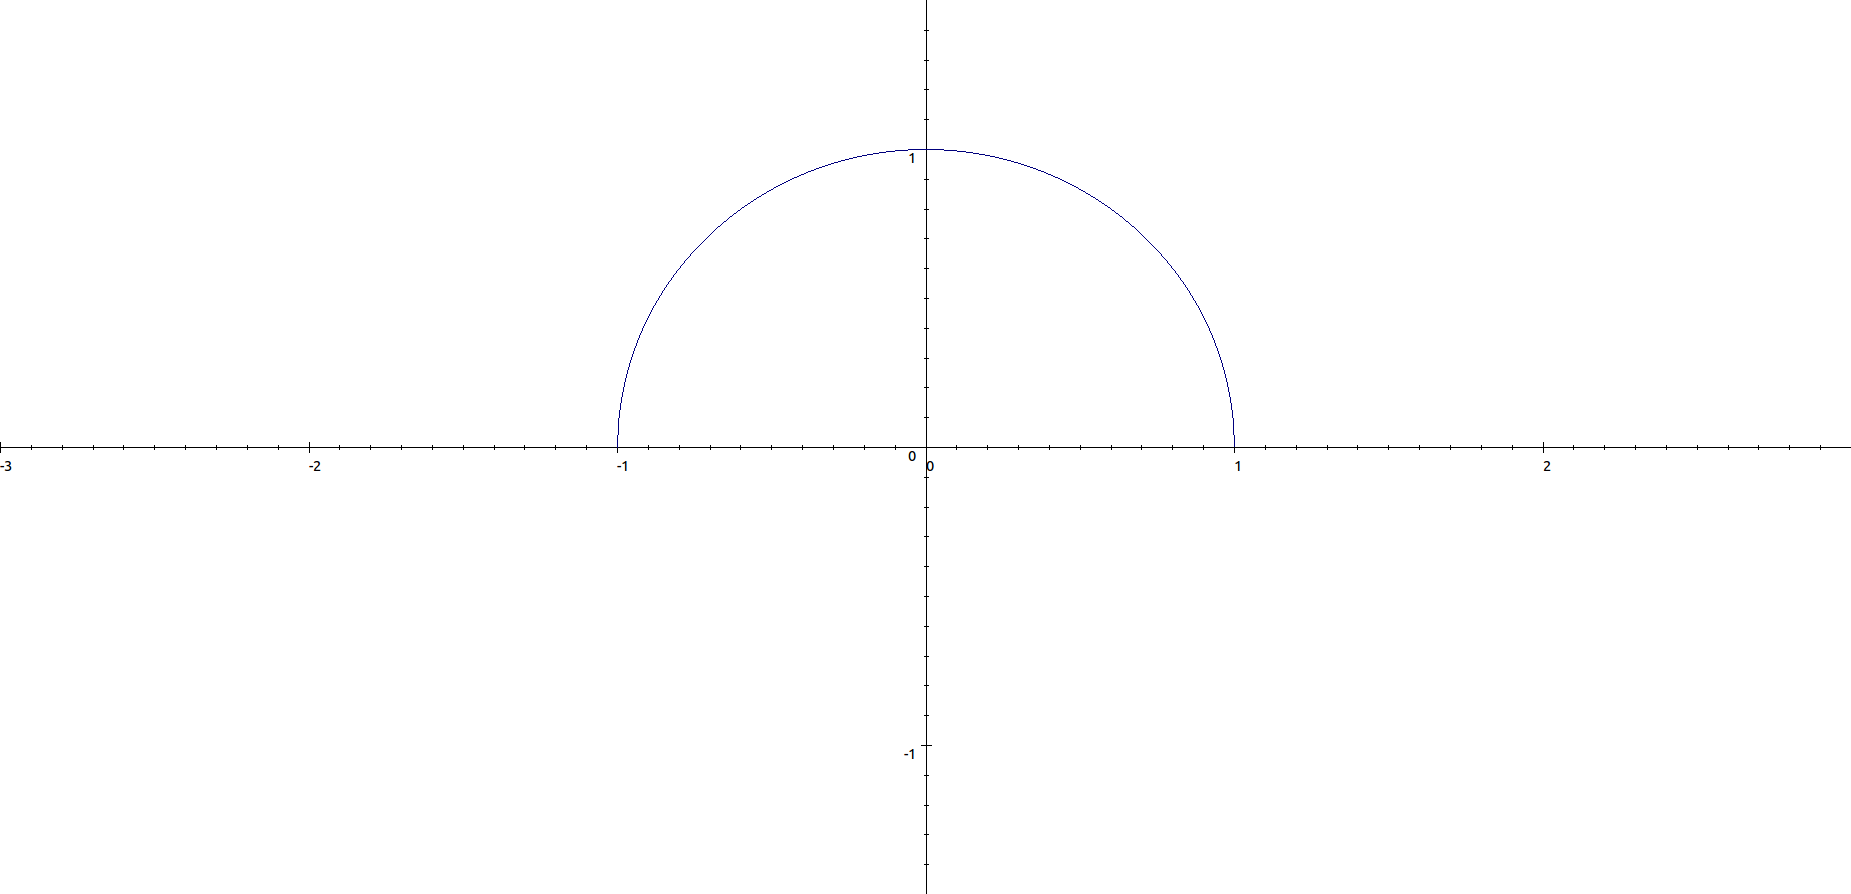
\includegraphics[scale=0.2]{circle}
		\caption{Plot of $\sqrt(1 - x^2)$ from -1 to 1}
	\end{figure}

	*sigh* it is only a half circle. Must have been the square root that messes it up. But whatever, we can work with that -- it still has exactly half of the area of a circle. Now to estimate the area under this half circle we can use small rectangles under the curve. How many of them depends on how accurately we want to know the value of $\pi$. Doing it by hand would get really tedious with any large number of rectangles, so we use the almighty computer to do the tedious calculations for us! We can use the following Python 3 code to run and print the answer: 
	\begin{figure}[H]
		\begin{lstlisting}
		
		def riemann_sum(a, b, n):
		"""	Numerical calculation of definite integral,
			starting from a and ending at b,
			with n rectangles. """
			
			def f(x):   return sqrt(1-x**2)	# Define half circle
			
			sum = 0					# Initialize variable for the area
			i = a						# We start at point "a"
			width = float((b - a)/n)	# width of every rectangle
			while i <= b:		# While the end point has not been reached
				sum += f(i) * width		# Add the areas of the rectangles
				i += width				# Keep track where we are
				
		return sum
		
		pi_over_two = riemann_sum(-1, 1, 1000000)
		print("\n\nNumerical calculation of integral under half circle with 1 000 000 rectangles:", pi_over_$
		"Gives us pi of value:", pi_over_two * 2, "with error:", abs(pi_over_two * 2 - pi), '\n')
		
		\end{lstlisting}
	\end{figure}
	
	\begin{figure}
		\centering
		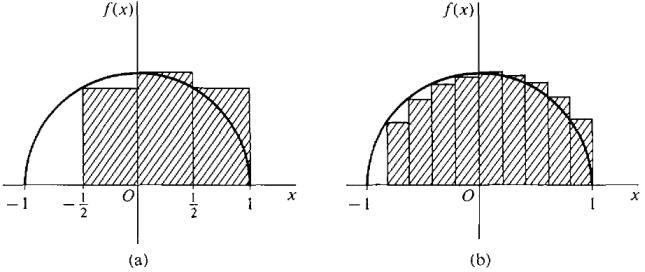
\includegraphics[scale = 0.4]{riemann_int_circle}
		\caption{Riemann integral under half circle with 4 and 10 rectangles. Code has a million thus giving a lot better estimate}
	\end{figure}
	
	This is a numerical method for giving an estimate for the definite integral: $$\int_{-1}^{1}\sqrt{1-x^2} = \frac{\pi}{2}$$
	
	It is just the area under the curve but looks scary and complicated. You can think of ways to improve the method -- or just don't bother and search the internet.



	\chapter{Mathematics celebrities}
	
	\section{Numbers}
	
	Mathematics doesn't have to be about numbers but for large number of topics you can't get by without quantifying with numbers what you are talking about. The numbers talked about here are either solutions to some problems or just make your life easier by making the solving step of a problem easier to handle. The later might be caused by number having distinct properties.\par
	
	\subsection{Can't have math textbook without $\pi$}
	
	Notorious number $\pi$ is known to many and hated by many for its presence in many aspects of trigonometry and loved by some for its extreme appearances in the most unexpected places including normal distribution equation, complex analysis and prime number theory. But also outside of mathematics, in physics the $\pi$ is present mostly in the form of a sphere or circle constant, for example: Coulombs law $F =\frac{Kq_1q_2}{4\pi\epsilon_0}$ describing the force 
	
	\subsection{Euler's number \textit{e}}
	Whenever someone is talking about naturally occurring exponential decay or growth there is a good chance we have this number lurking around. If there is a need for a well behaved derivative; \textit{e} should be first thing that pops to your head.
	\subsubsection{Limit definition and origin}
	The constant itself was found when Jacob Bernoulli tried to find value of the following expression $$\lim_{n\rightarrow\infty} (1 + \frac{1}{n})^n$$
	This was encountered when Bernoulli was studying compound interest and can be demonstrated with a thought experiment where you wish to lend a dollar to the bank. In order to keep it simple lets imagine that you are expecting to get 100 \% profit from a one year period. Meaning that at the end of the year you expect to get back 2 dollars. If you wish to earn a bit more money you could ask the bank to return your investment on half year and reinvest all your money. In that case you would get back 2.25 dollars which is essentially gaining money from nothing. Now, if you want to find a formula for dividing the year into $n$ pieces, cashing out and reinvesting every $\frac{1}{n}$'th of the year you end up with profit of $(1 + \frac{1}{n})^n$ dollars. The whole difference between this and the equation beforehand is the "$\lim_{n\rightarrow\infty}$" which is the math way of saying lets look as $n$ gets really big. Bernoulli without the help of calculators settled with approximate value of 2.5. Which is good enough for many applications.
	\subsection{Why am \textit{i} here?}
	
	\subsection{Pearl of mathematics}
	$$e^{i\pi} + 1 = 0$$
	Combining all of the above numbers in an identity gives us an equality which is often called the most beautiful equation.
	\subsubsection{Advanced: Proof through Taylor expansions}
	As a reminder, Taylor series is a way of expressing functions through their change. Taylor series is an infinite polynomial expression converging to original function $f$ around a \textit{pivot point} $a$. Taylor series is defined to be:
		$$f(x) = \sum_{n=0}^{\infty} \frac{f^{(n)}(a)}{n!}(x - a)^n$$
	Meanwhile some of most useful and used Taylor series expansions are:
		$$sin(x) = \sum_{n=0}^{\infty} \frac{(-1)^nx^{2n+1}}{(2n+1)!} = x - \frac{x^3}{3!} + \frac{x^5}{5!}...$$
		$$cos(x) = \sum_{n=0}^{\infty} \frac{(-1)^nx^{2n}}{(2n)!} = 1 - \frac{x^2}{2!} + \frac{x^4}{4!}...$$
		$$e^x = \sum_{n=0}^{\infty} \frac{x^n}{n!} = 1 + x + \frac{x^2}{2!} + \frac{x^3}{3!}...$$
		
	Taylor series can be thought of as a way of expressing function through its change instead of its values at every point. This is expressed by the need of $n$'th derivative. \newline
	
	Now define x to be multiplied by constant of i, another way to write it down: $x \defeq i x$. Then plug it in the $e^x$ Taylor series gives us:
		$$e^{ix }= \sum_{n=0}^{\infty} \frac{(ix)^n}{n!} = 1 + ix + \frac{(ix)^2}{2!} + \frac{(ix)^3}{3!}...$$
	
	Using identity of $i^2 = -1$ we can simplify this expression to:
	
		$$e^{ix} = \sum_{n=0}^{\infty} \frac{(ix)^n}{n!} = 1 + ix - \frac{x^2}{2!} - \frac{ix^3}{3!} + \frac{x^4}{4!} + \frac{ix^5}{5!}...$$
	
	Combining terms with i and factoring it out yields us with two Taylor series which can be noticed to be equal to the Taylor series of sine and cosine:
	
		$$e^{ix} = \sum_{n=0}^{\infty} \frac{(ix)^n}{n!} = i(x -  \frac{x^3}{3!} + \frac{x^5}{5!}...) +  (1 - \frac{x^2}{2!} + \frac{x^4}{4!} ...) = isin(x) + cos(x)$$
		
	Then setting a value for x; $x \defeq \pi$
		$$e^{i\pi} = cos(\pi) + isin(\pi) = -1$$
		
	Rearranging the terms gives us back what we set out to find:
		
		$$e^{i\pi} + 1 = 0$$
	
	\section{Equations}
	
	\subsection{Normal distribution}
	\subsection{Fourier transform}
	\subsection{Chaos theory}
	
	\subsubsection{Nobody knows if this is the introduction}
	
	Chaos theory is fairly recent topic on the field of mathematics and was mostly developed to explain the failure of numerical calculations in models. If there is some small error (usually by default $10^{-8}$) due to limited precision of computers the error might cumulate and produce dramatically different results. 
	
	\subsubsection{Lemming population}
	
	Lemmings are rodents that have long-standing misconception that they perform mass-suicides after every few years. The theory goes that if the population is too numerous they try to migrate and drown themselves in masses into bodies of water. The theory seemed very plausible due to very high fluctuations in the lemming population over the years. It turns out that it is not due to suicidal thoughts but rather inherent dynamics of the system. \par
	
	Thinking about the change in lemming numbers is a lot easier than trying to describe the lemming numbers directly. Important part of the model is the maximum number of lemmings environment can sustain, lets call that $M$. We will denote the current number of lemmings with $N$ and time with $t$. Very important is also the reproduction constant $r$ which denotes average number of offspring per lemming. \par
	
	So we are looking for a formula for the rate of change in the number of lemmings $\frac{dN}{dt}$. It should depend on the number of lemmings born in a time interval, that is just $rN$. And the number of lemmings that dies due to environment being over-crowded -- $rN\times\frac{N}{M}$. This gives us that the change is: $$\frac{dN}{dt} = rN(1 - \frac{N}{M})$$
	
	While the reproductive rate of lemmings can be empirically measured and is around 3.61.
	
			Running the simulation twice with initial lemmings 100 (blue) and 110 (red) produces these results:\newline
	\begin{figure}[H]

		\centering
		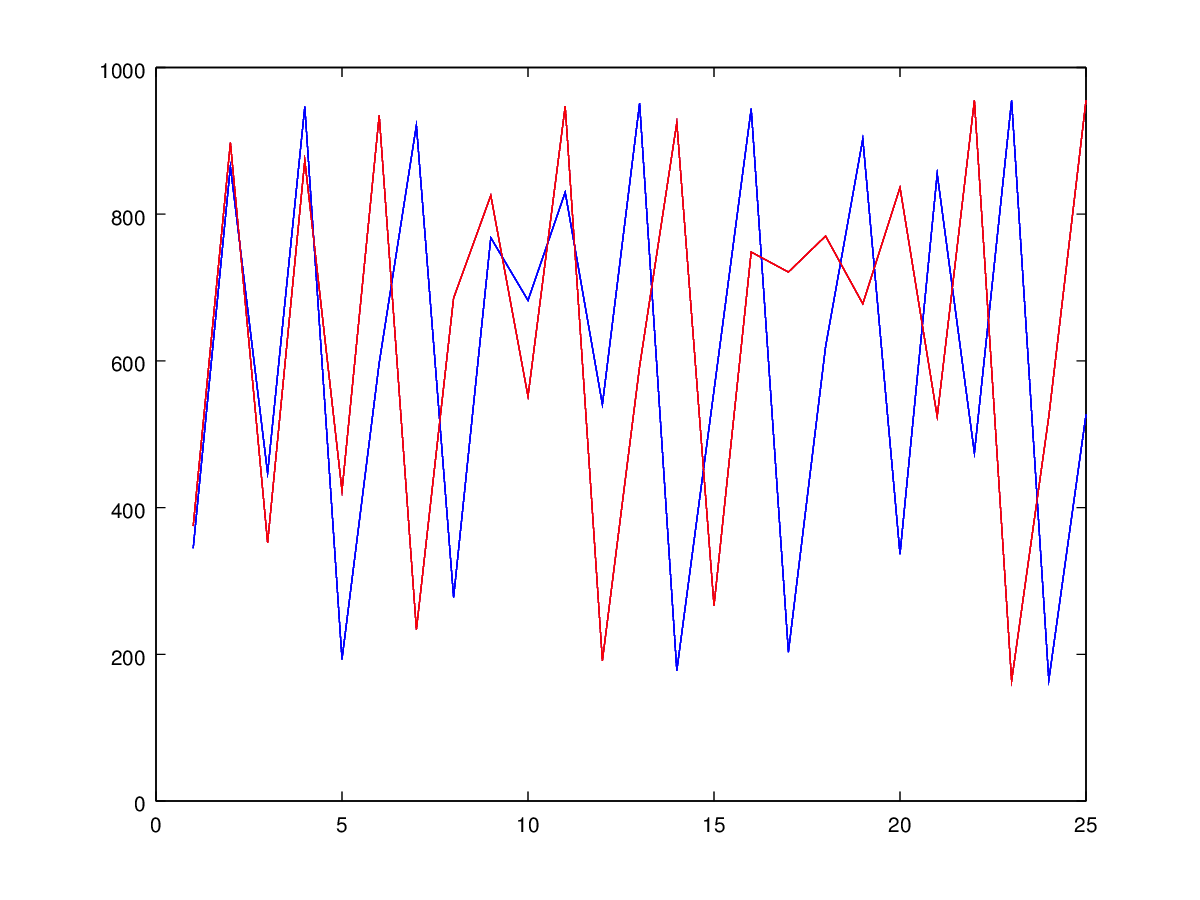
\includegraphics[scale=0.6]{lemmings.png}
		\caption{Lemmings population dynamics with initial conditions 100 and 110}
	\end{figure}
	
	We can see that the lemming populations alternate wildly between high number and very few lemmings. Also we can see that both red and blue plots start out together but with minor change in the initial conditions they diverge from each other quick. That is 
	
	%history = log_growth(100, 3.83, 1000, 25)
	%history2 = log_growth(110, 3.83, 1000, 25)
	%plot(history); hold on; plot(history2, 'r');
	
	
	\subsubsection{May's logistic map}
	
	\chapter{Models: Complexity from simplicity}
	
	\section{Cellular Automaton}
	
	\subsection{Elementary cellular automaton}
	\subsubsection{Introduction}
	Cellular automaton are systems which consist of cells which are next to each-other in regular pattern which all have one of finite number of states and a fixed rule according to which the cell states are changed.
	
	In the case of elementary cellular automaton the grid consists of squares and the model itself is one-dimensional. Meaning that
	


\begin{center}
	\begin{tabular}{ |c|c|c| } 
		\hline
		cell1 & cell2 & cell3 \\ 
		cell4 & cell5 & cell6 \\ 
		cell7 & cell8 & cell9 \\ 
		\hline
	\end{tabular}
\end{center}


	\subsubsection{New kind of science}
	\subsection{Game of life}
	\subsection{Schelling's segregation model}
	
	\section{State machines}
	
	\subsection{Transitioning here}
	
	State machines are models in which you have certain probabilities to transfer from one group to another. Sometimes the question is framed to an individual but more often it is even more interesting to see where would groups of people tend to move in these systems. They can be played out as simulations or on some occasions there exists set of obtainable equations that describe the internal dynamic. There are two types of simulation that can be done here, either agents moving between states are discrete or they also can be real valued.
	
	\subsection{SIS model}
	
	Susceptible-Infected model is about epidemiology -- study of diseases in defined populations (e.g flu outbreak in your school or workplace). This model has two states, lets call them S and I. There is some probability that Susceptible person will become Infected, lets call that $\alpha$. The probability that Infected person will get back into Susceptible group is $\beta$. This can be shown on the graph as follows:
		\begin{center}
			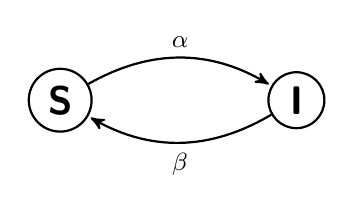
\begin{tikzpicture}[->,>=stealth',shorten >=1pt,auto,node distance=3cm,
			thick,main node/.style={circle,draw,font=\sffamily\Large\bfseries}];
			
			\node[main node] (1) {S};
			\node[main node] (2) [right of=1] {I};
			
			\path[every node/.style={font=\sffamily\small}]
			(1) edge [bend left] node [bend right] {$\alpha$} (2)
			(2) edge [bend left] node [bend left] {$\beta$} (1);
			
			\end{tikzpicture}
		\end{center}
	

	But that is not all! Imagine a situation that for there are 100 people in a room and none of them is sick. Then nobody should ever become sick, but naive approach to our current model would suggest that probability $\alpha$ is always occurring. Therefore the transition rate must depend on the amount of infected people I. Now think of the situation where there are 100 sick people in a room. As long as none of them gets well there is no possibility of any people becoming sick. Therefore it must also depend on the amount of susceptible people in the room.
	Therefore the amount of people becoming sick at any moment can be described by $\alpha S I$. \par
	
	Now moving to the people who are in Infected group, get well and move back to Susceptible group. You can take a moment to convince yourself (via similar argumentation to above) that that only depends on the amount of people in Infected group. Meaning that the amount can be described by $\beta I$.\par
	
	Now if we want to know the change $(\frac{dS}{dt})$ of people in group S it is the amount of people going in minus the amount of people going out, by the same argumentation we find change in group I ($\frac{dI}{dt}$): $$\frac{dS}{dt} = \beta I - \alpha S I $$ $$ \frac{dI}{dt} = \alpha S I - \beta I$$
	
	Now we are in a place where we can set initial conditions (how many susceptible and infected people we start out with) and then iterate over the \textit{change equations} to find what happens!	

	\begin{figure}[H]
		\centering
		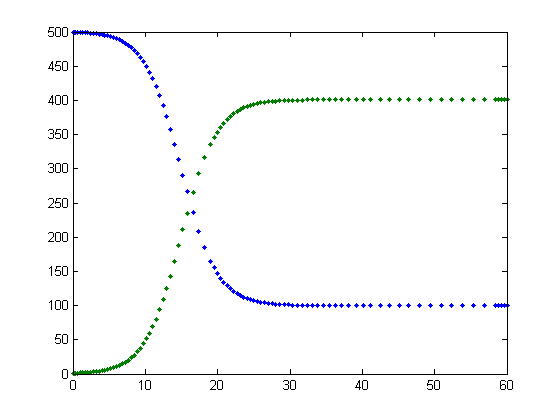
\includegraphics[scale=0.7]{SISeq}
		\caption{Blue - Suseptible, Green - Infected; CITATION}
	\end{figure}
	% https://en.wikipedia.org/wiki/Compartmental_models_in_epidemiology#/media/File:Sissys.png
	
	This graph shows that the model reaches equilibrium by around 30 on the time axis, this might differ according to initial conditions.
	
	\subsubsection{Advanced: SIS model analytical solution}
	
	For a simple model like SIS there often is an analytical solution. Within this chapter I hope to show the derivation of the solution.
	
	We start with boundary condition $S + I = k$. The whole population is always constant which is arbitrary positive number k. To remind, the differential equations were: $$\frac{dI}{dt} = \alpha S I - \beta I $$ $$ \frac{dS}{dt} = -\frac{dI}{dt}$$
	
	Substituting $S = k - I$ to first differential equation. leaves us with $\frac{dI}{dt} = \alpha (k - I) I - \beta I = \alpha k I - \alpha I^2 - \beta I$
	
	\subsection{SIR model}
	
	Instead of the SIS, the SIR model contains three groups of people: Susceptible, infected and recovered. Recovered group contains people that can never again become infected because they have immunity. The state graph looks like this:
				\begin{center}
					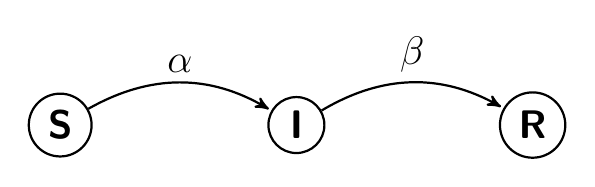
\begin{tikzpicture}[->,>=stealth',shorten >=1pt,auto,node distance=3cm,
					thick,main node/.style={circle,draw,font=\sffamily\Large\bfseries}];
					
					\node[main node] (1) {S};
					\node[main node] (2) [right of=1] {I};
					\node[main node] (3) [right of=2] {R};
					
					\path[every node/.style={font=\sffamily\Large\bfseries}]
					(1) edge [bend left] node [bend right] {$\alpha$} (2)
					(2) edge [bend left] node [bend right] {$\beta$} (3);
					
					\end{tikzpicture}
				\end{center}
				
	The argumentation for change equations is almost identical to SIS model except there is no people ever joining susceptible group and none are ever leaving recovered. Change equations are:
	
	$$\frac{dS}{dt} = -\alpha S I$$
	$$\frac{dI}{dt} = \alpha S I - \beta I$$
	$$\frac{dR}{dt} = \beta I$$
	
	Iterating over time gives us a graph:
		\begin{figure}[H]
			\centering
			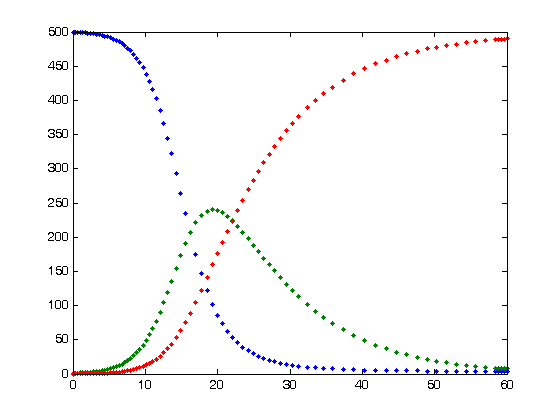
\includegraphics[scale=0.7]{SIReq}
			\caption{Blue - Suseptible, Green - Infected, Red - Recovered; With initial conditions of $S = 500$, $I = 1$, $R = 0$. CITATION}
		\end{figure}
	
	\subsection{Cellular approach to SIR}
	
	Now if we define a grid and populate it with susceptible people according to population density in a given area (E.g local city, state, country or even the whole world. You can find the density maps online.) Here is population density of france: 
	
	\begin{figure}[H]
		\centering
		\includegraphics[width=7.5cm, height=7.5cm]{france_density}
		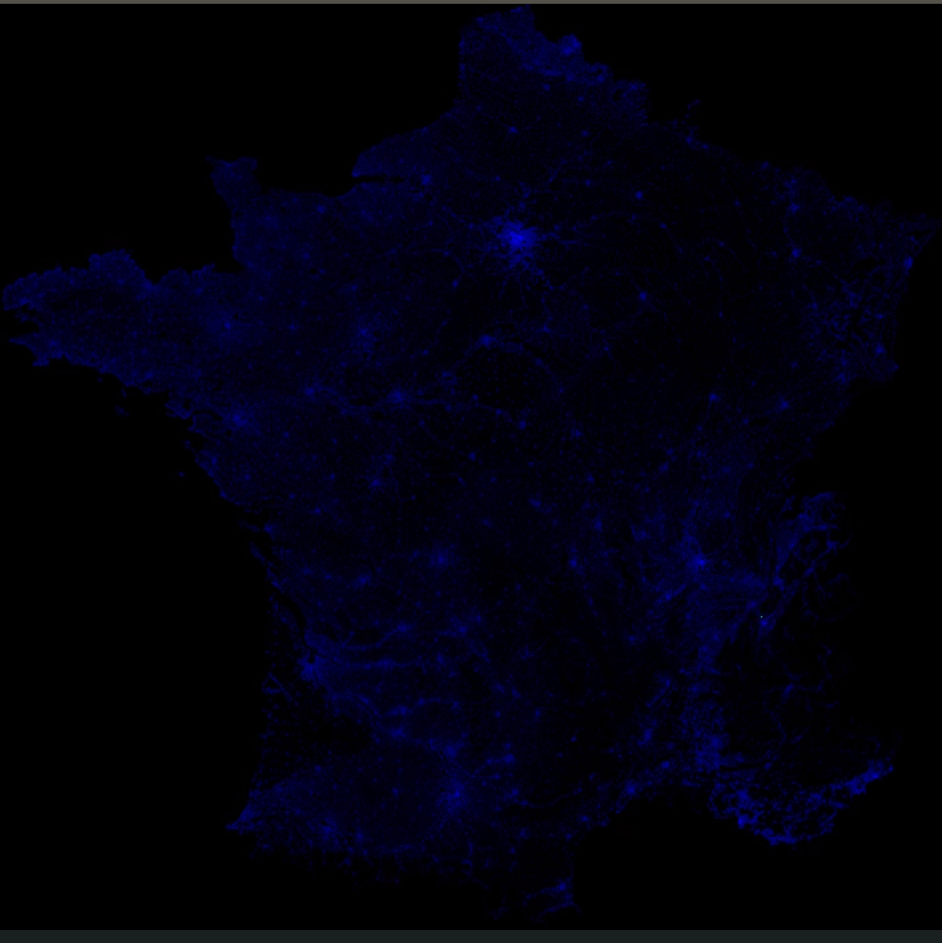
\includegraphics[width=7.5cm, height=7.5cm]{france_density_SIR}
		\caption{First one is raw data, second one is already placed in a 400x400 grid}
	\end{figure}
	 This makes it possible to bring the simulation to next level. Making the cell able to interact with the population in neighboring cell gives you a very good model of what happens in the real world -- you are likely to only infect people near you. Also from here on you can go wild with the features you can add: government intervention policies, transport routes, infection constants according to location etc. Every single iteration of thought process giving an even more difficult model to comprehend and predict but also closer to the real life. Math wizardry in action. But now lets look at some pretty pictures from simulations.
	\section{Agent based models}
	
	Agent based models are probably one of the easiest ones to conceptualize but bring many interesting results. The models are constructed of independent agents that interact with the surroundings and often with each other according to some set of rules.
	
	\subsection{Standing ovation model}
	
	Standing ovation model tries to capture group behavior from influence of others. The toy example here is people deciding to stand and clap or not to stand after an theater show. Understanding this toy example can lead to understand the uprising mechanics and why they are so hard to predict. Also formalizing your ideas on paper will make you understand what pieces of information you need and what is the least viable model you can use.
	 
	\subsection{Examples of artificial evolution }
	
\end{document}